%----------------------------------------------------------------------------
\chapter{Evaluation}
%----------------------------------------------------------------------------
This chapter presents the applicability of the designed framework, evaluates its current capabilities and points out improvement possibilities. Section \ref{sec_theoeval} evaluates the current state of the framework, then Section \ref{sec_casestudy} presents a case study about the applicability of our solution. Lastly, Section \ref{sec_futurework} presents the opportunities for the continuation of the work.

%----------------------------------------------------------------------------
\section{Theoretical Evaluation} \label{sec_theoeval}
%----------------------------------------------------------------------------

\clearpage
%----------------------------------------------------------------------------
\section{Case Study: Pedestrian Crossing} \label{sec_casestudy}
%----------------------------------------------------------------------------
This section demonstrates the capabilities and limitations of the framework. It presents a problem commonly modeled using state-based models, which is complex enough to demonstrate all aspects of the designed Interactive Learning Entity, but also simple enough to solve - thus verify - only using some background knowledge and common sense. [TODO ref gamma tutorial?]

%---------------------------------------------------------------
\subsection{Introduction} \label{subs_casestudyintro}
%---------------------------------------------------------------

The problem to solve is modeling a pedestrian crossing with a standard traffic light and a pedestrian light as illustrated on Figre \ref{fig_casestudy_systemstates}. As the traffic lights and the pedestrian lights on the opposite sides of the crossing behave identically, we are going to model only one instance of each device. 

The traffic light is looping through the red-green-yellow-red sequence. As an extra, there is an interrupted mode that may be triggered by the police, which results in blinking yellow light. The pedestrian light loops through the red-green-red sequence, and turns black when an interrupt arrives. A subsequent interrupt turns the lights back on, also considering that the sytem must always be in a safe state - i.e. the lights must not allow passage for both the pedestrians and the road vehicles at the same time.

\begin{figure}[!ht] 
	\centering
	\fbox{
		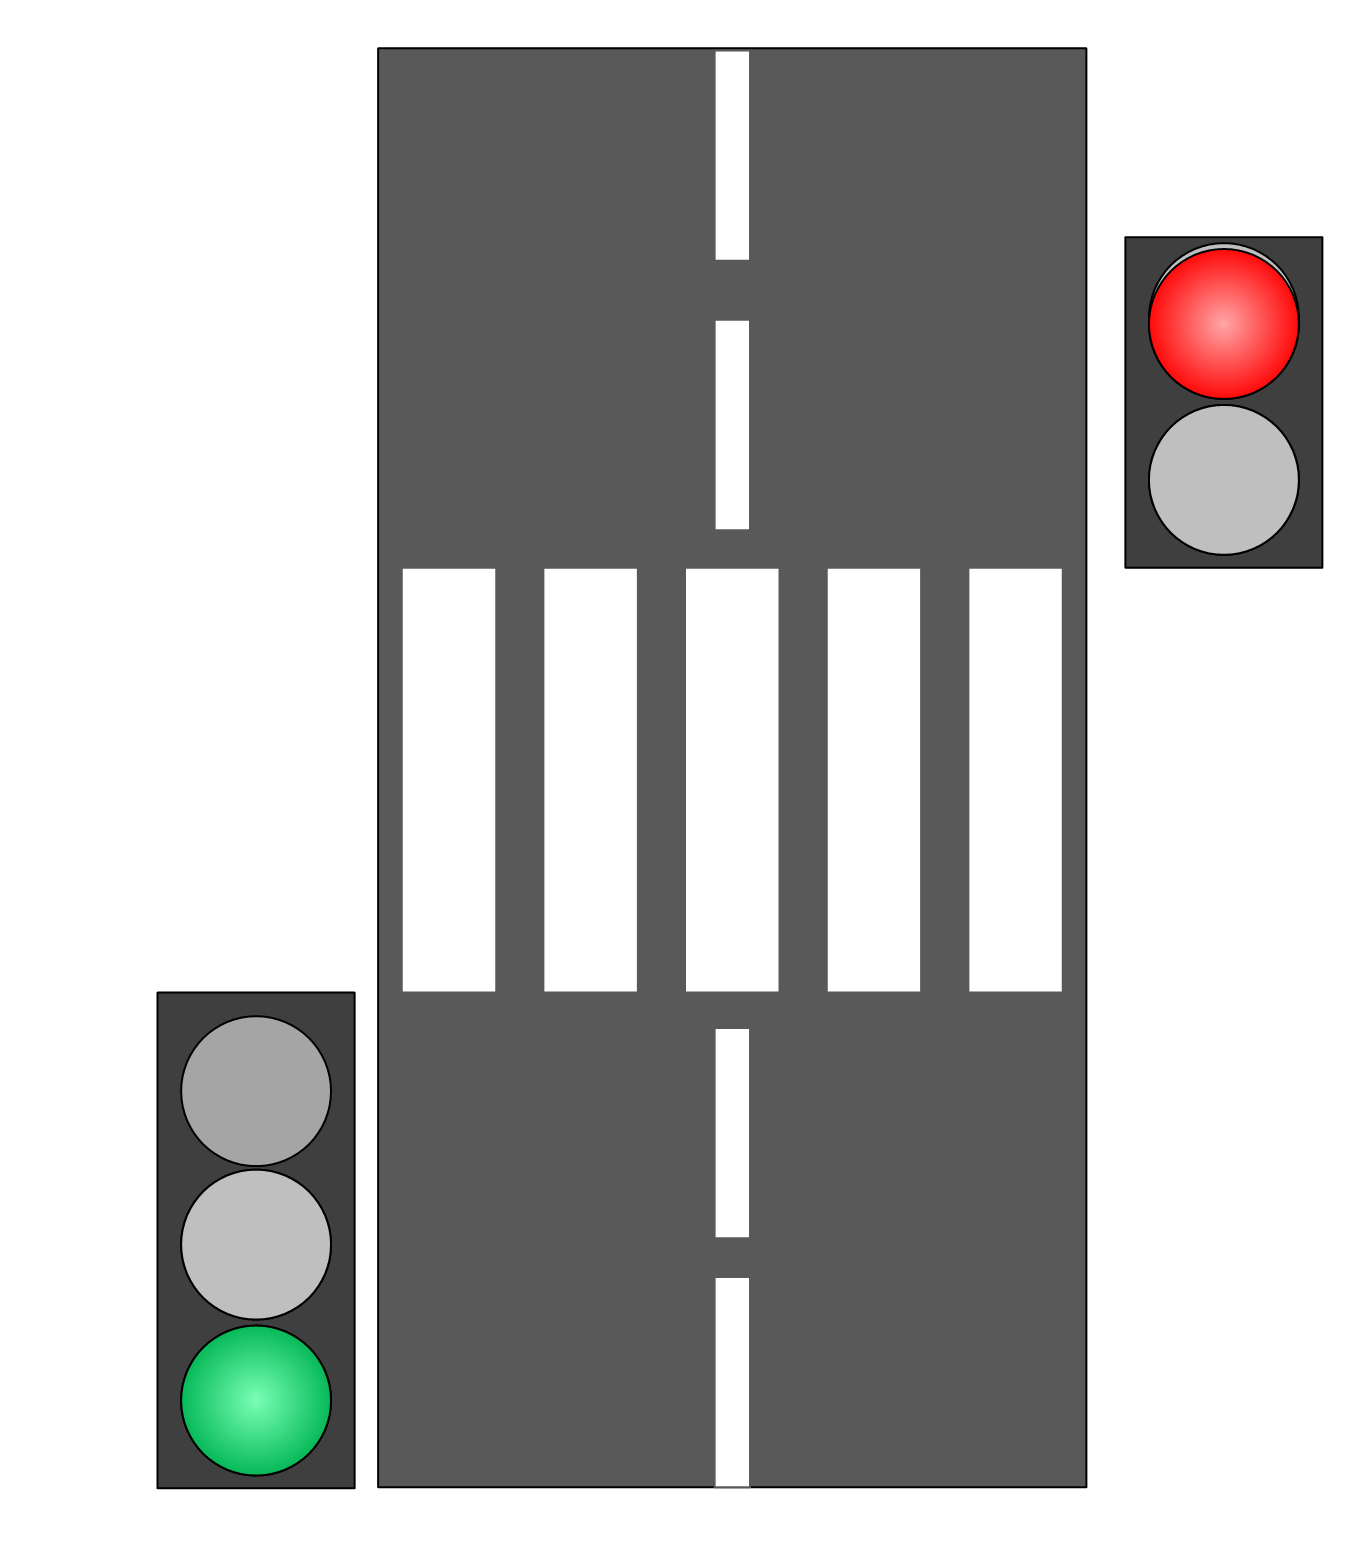
\includegraphics[width=30mm, keepaspectratio]{figures/casestudy_state1.png}
	}
	\fbox{
		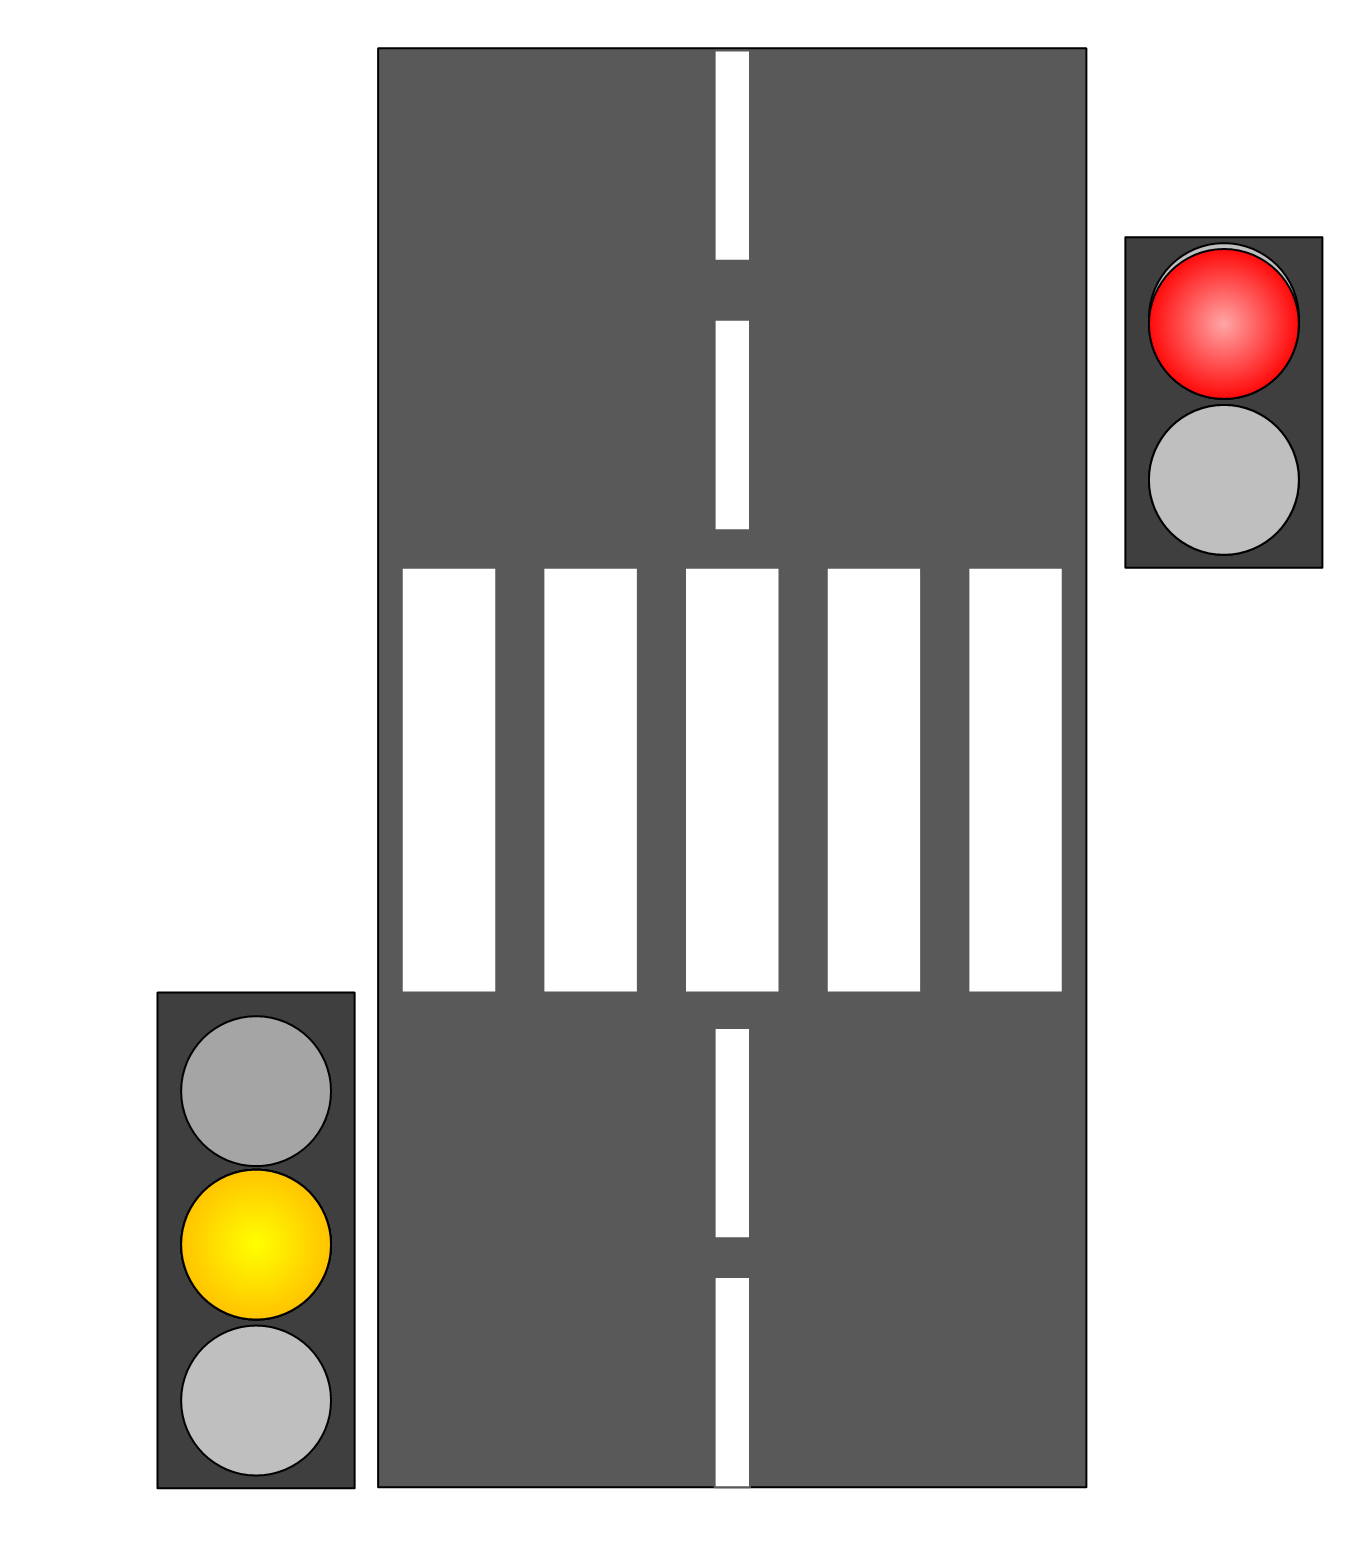
\includegraphics[width=30mm, keepaspectratio]{figures/casestudy_state2.png}
	}
	\fbox{
		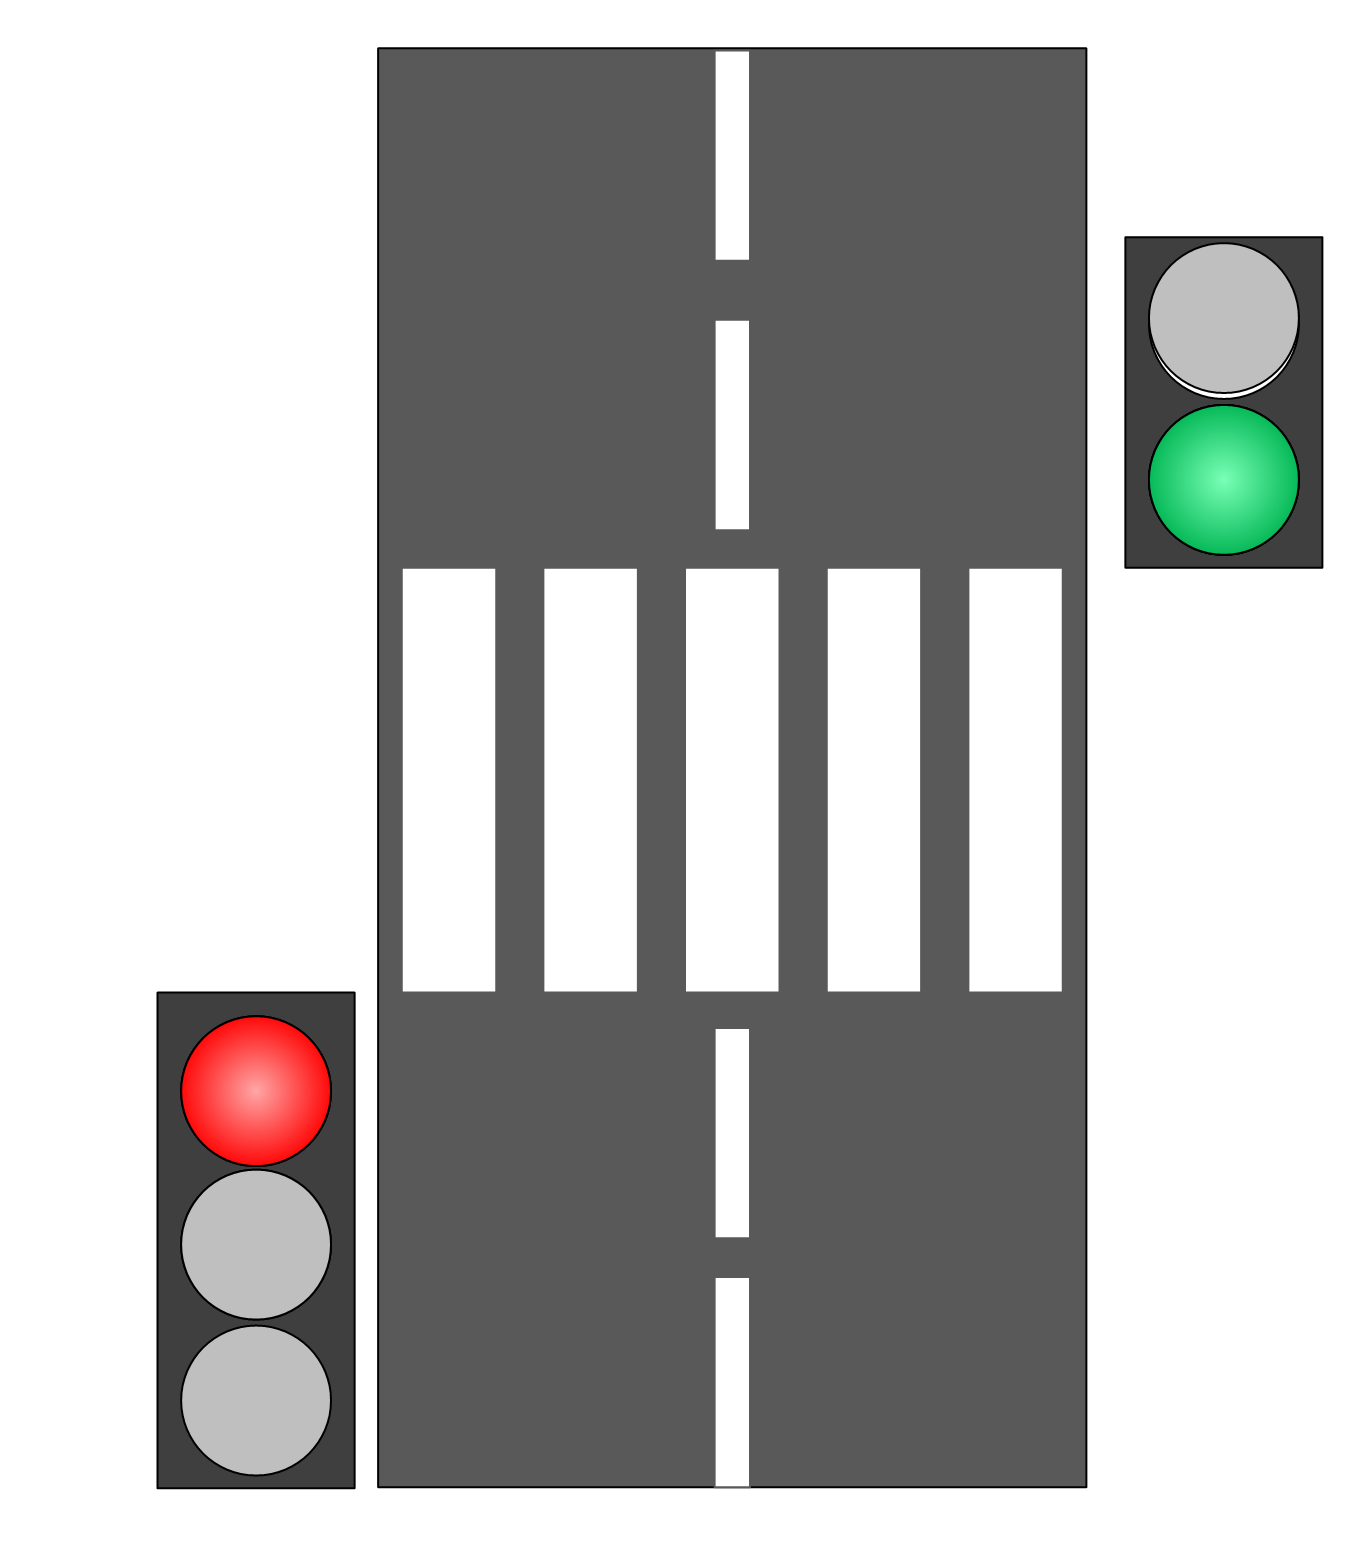
\includegraphics[width=30mm, keepaspectratio]{figures/casestudy_state3.png}
	}
	\fbox{
		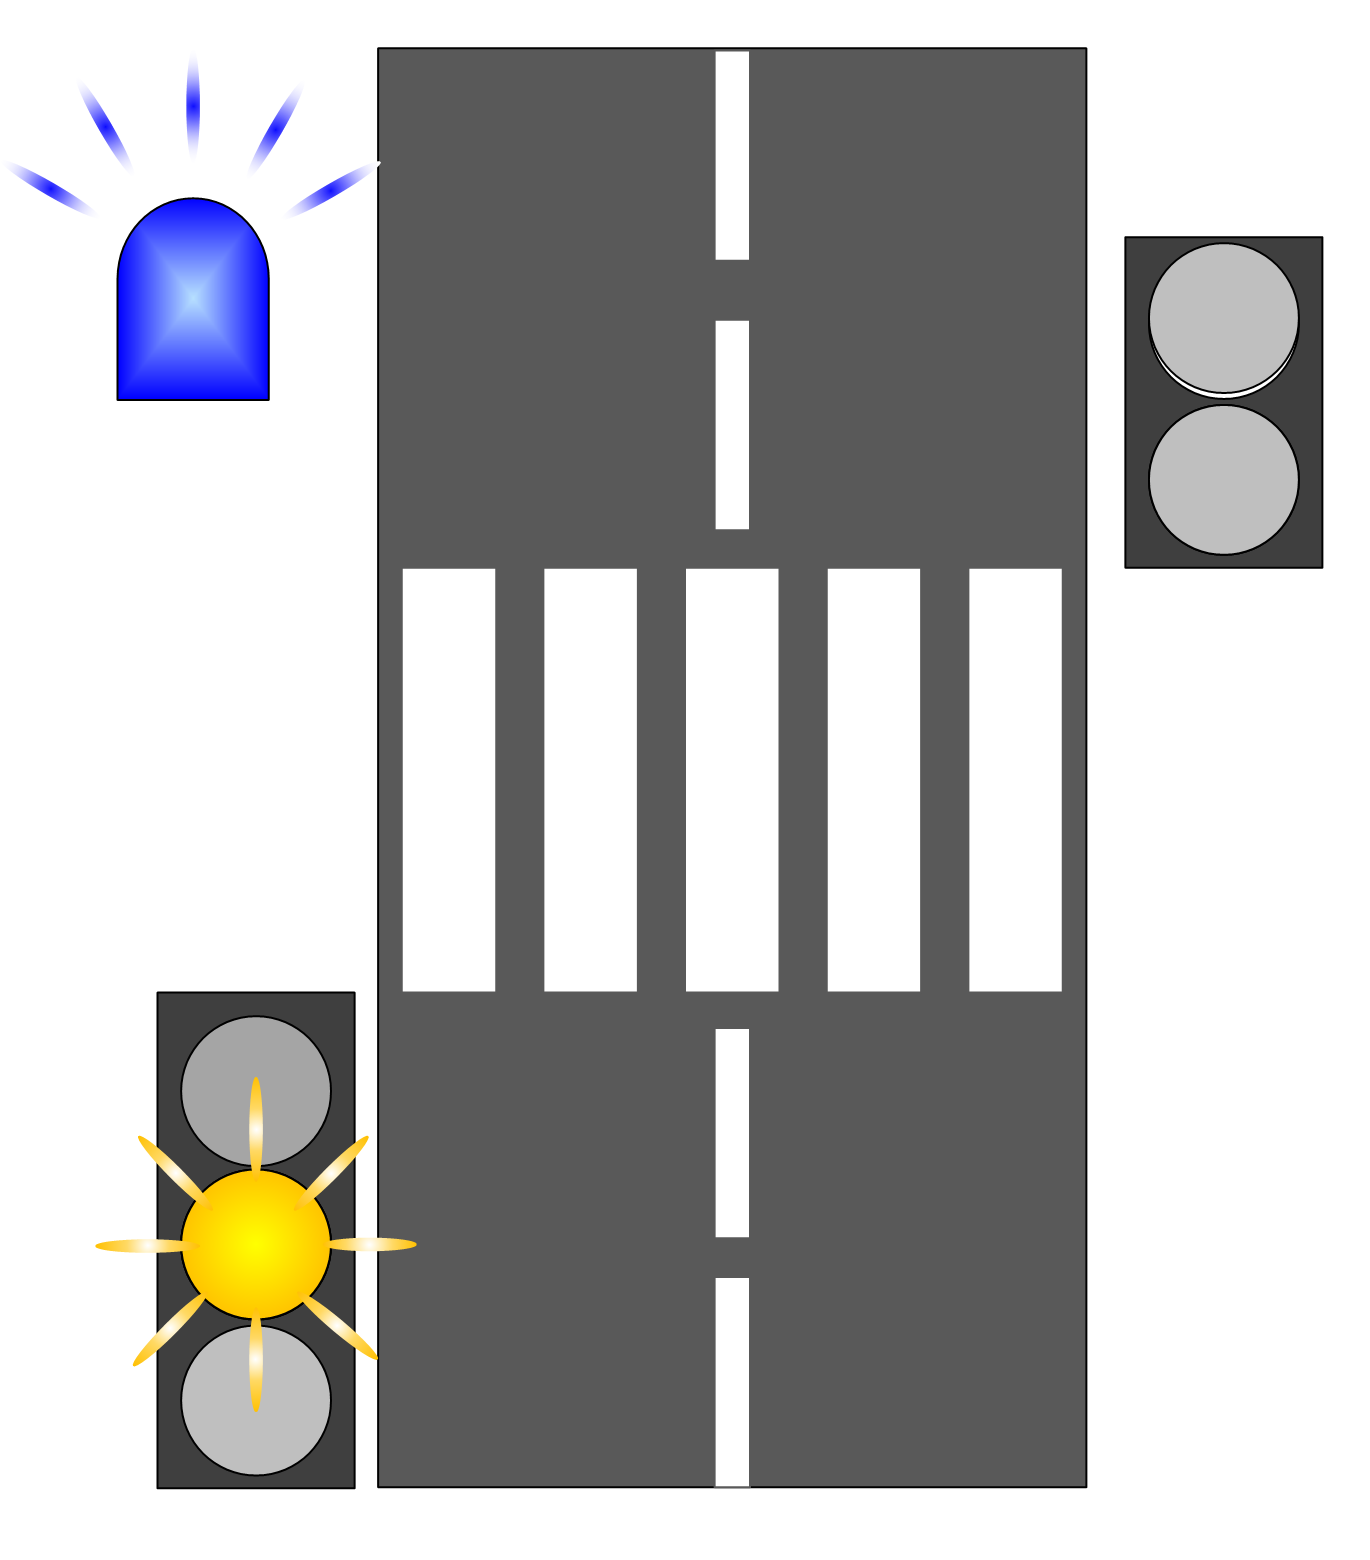
\includegraphics[width=30mm, keepaspectratio]{figures/casestudy_state4.png}
	}
	\caption{Possible states of the system: normal operation (\textit{three from the left}) and the interrupted state \textit{(right)}} 
	\label{fig_casestudy_systemstates}
\end{figure}

%---------------------------------------------------------------
\subsection{Component Design} \label{subs_casestudycomps}
%---------------------------------------------------------------

The previous subsection mentioned two components of the composite system: a traffic light and a pedestrian light. To realize the safe state of the system, the components must synchronize their behavior, justificating the existence of a third, controller component. The traffic and pedestrian light components should have one input and one output port -- they  are relatively simple -- and the controller should have an input port for the police and two output ports for the components.

\textbf{The traffic light component} has two possible inputs on its input port (TrafficControl) - toggle and interrupt - and four outputs on its output port (TrafficDisplay) - red, green, yellow and blinking yellow - as it appeared in the problem description.

\textbf{The pedestrian light component} has the same two inputs on its input port (PedestrianControl) - toggle and interrupt - and three outputs on its output port (PedestrianDisplay) - red, green, and black - as it appeared in the problem description.

\textbf{The controller component} controls the rhythm of the change of states and also interrupts the other components when the police interrupt arrives. TIt has an input port ('\textit{Police}') for the police interrupt and two output ports ('\textit{TrafficControl}' and '\textit{PedestrianControl}') - matching the input ports of the other components.

The described components and their connections are illustrated on Figure \ref{fig_casestudy_blockdiagram}.

\begin{figure}[!ht] 
	\centering
	%\fbox{
		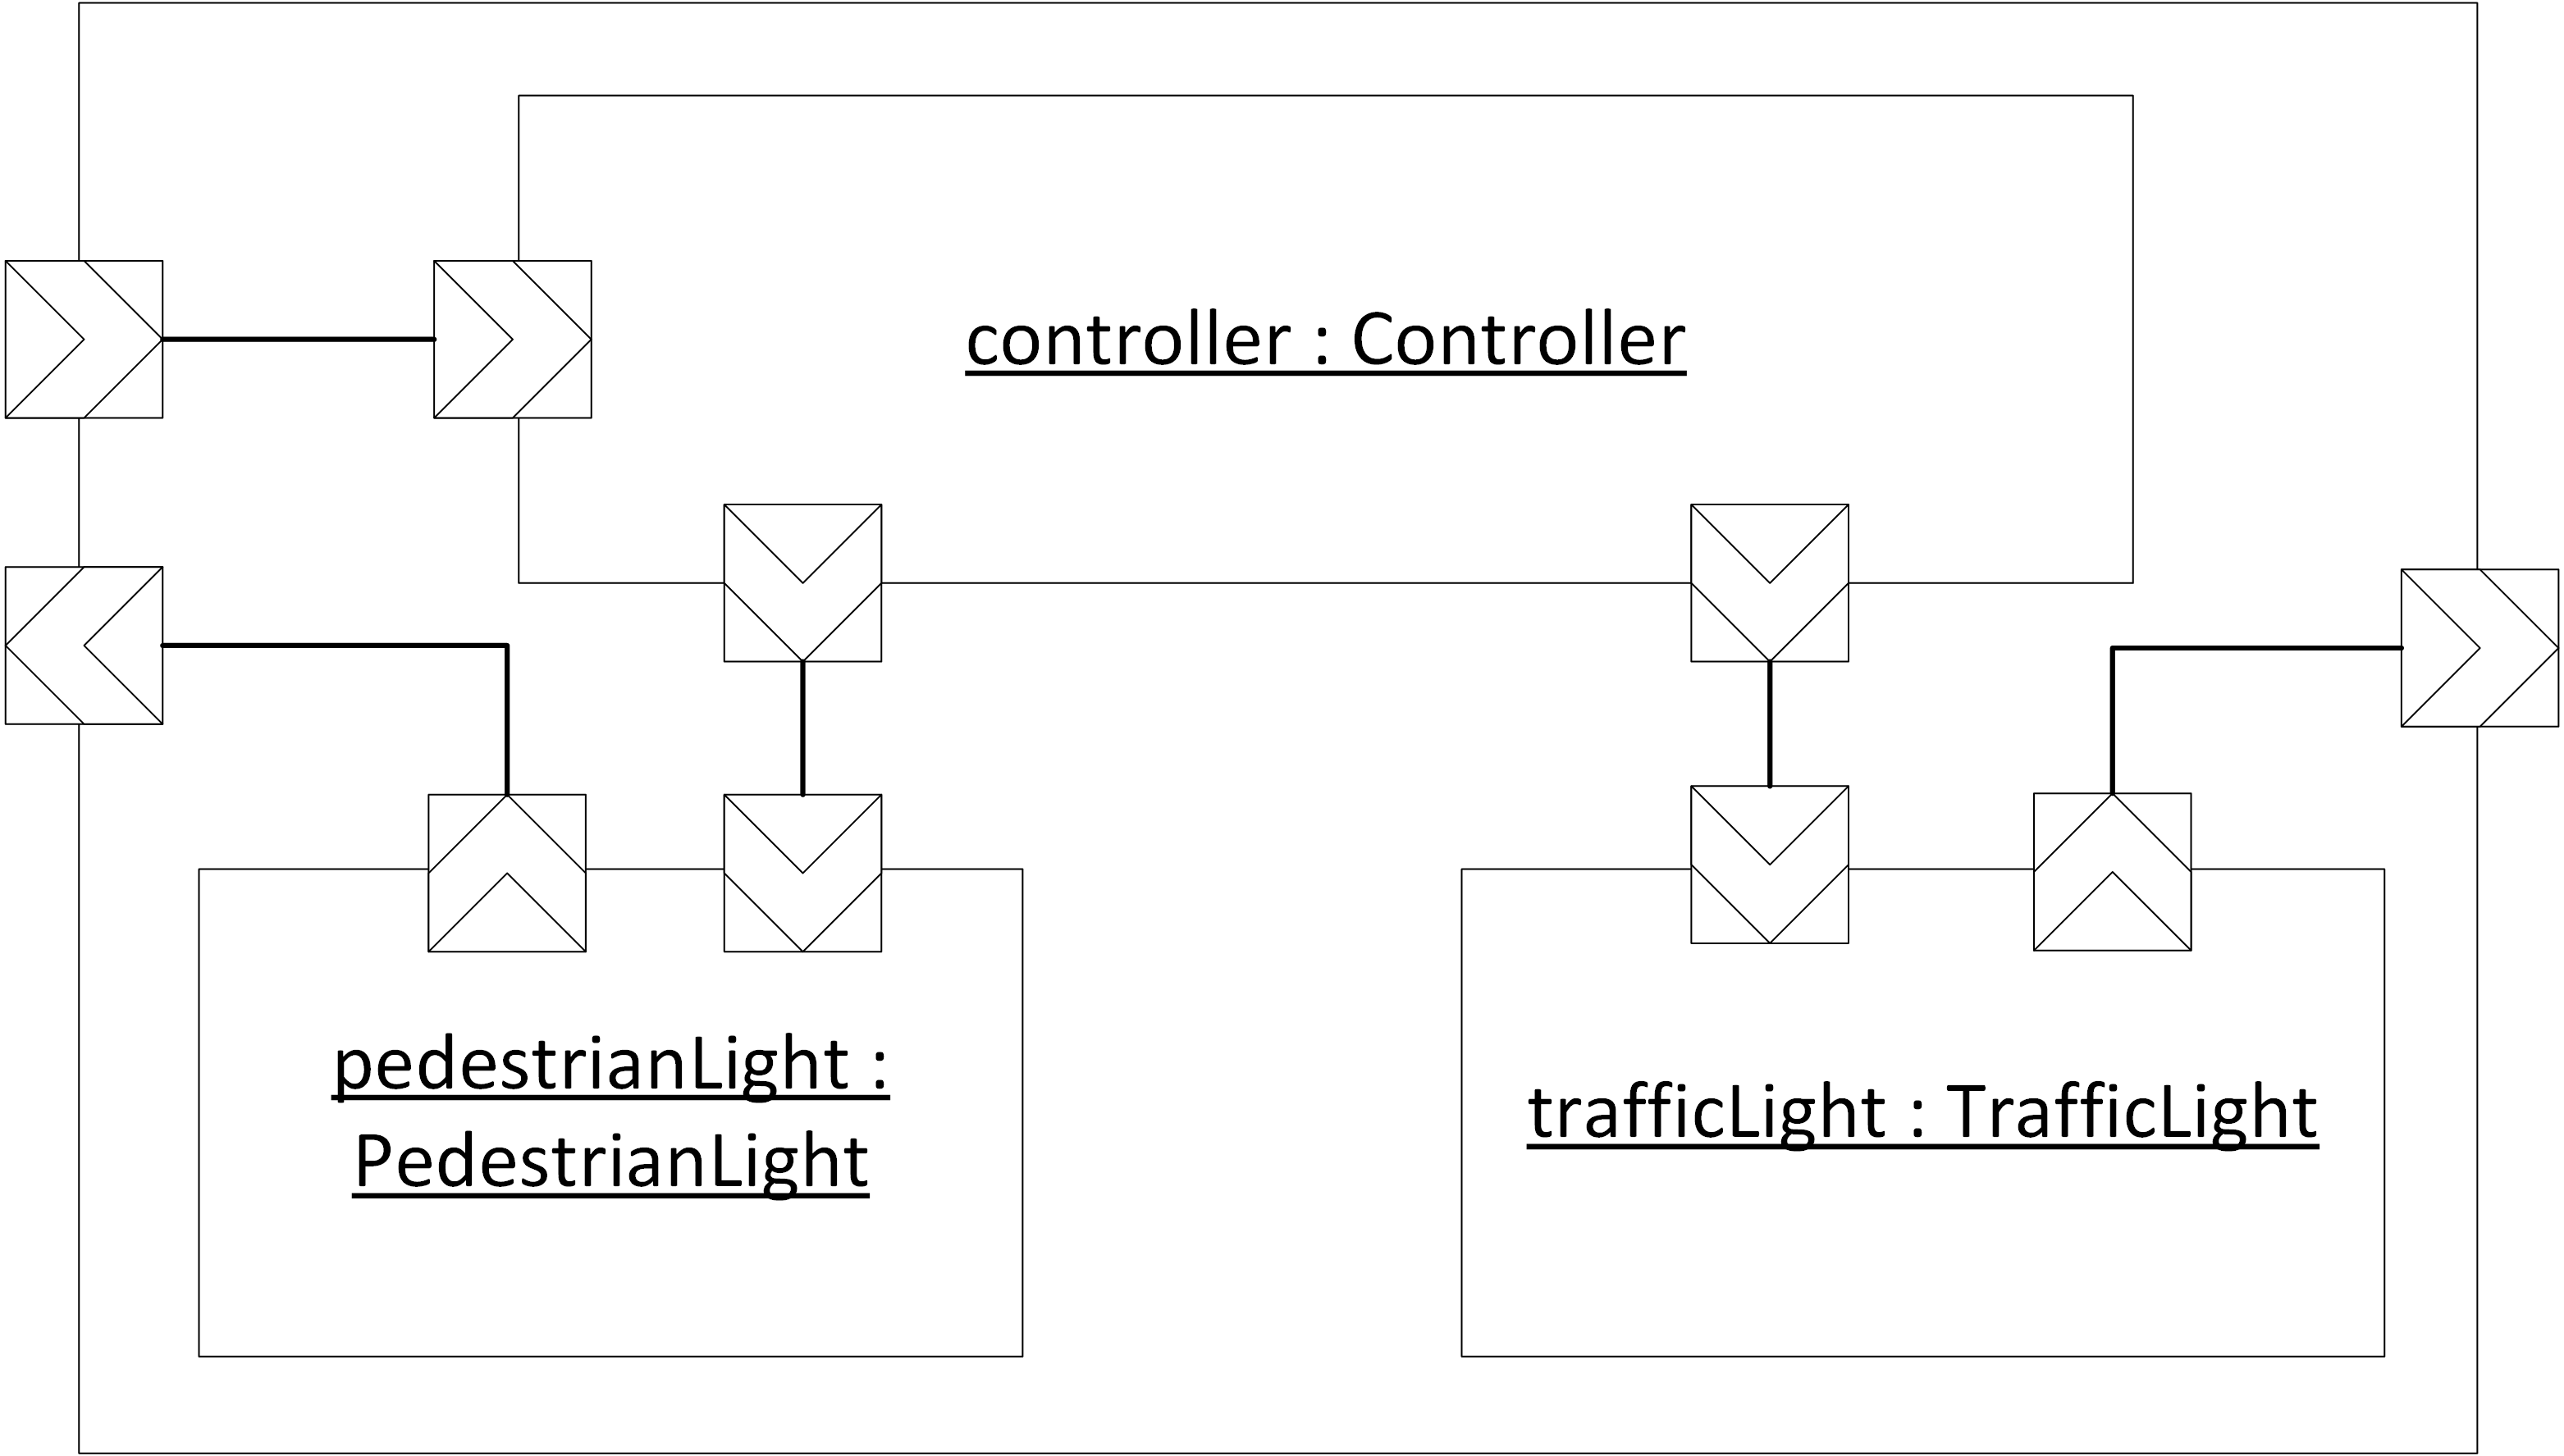
\includegraphics[width=130mm, keepaspectratio]{figures/casestudy_blockdiagram.png}
	%}
	\caption{Components of the modeled system and their connections} 
	\label{fig_casestudy_blockdiagram}
\end{figure}

\textbf{The Expected Behavior of the Components} 

TODO define requirements that fit the 'expected' statecharts below kinda formally.


%---------------------------------------------------------------
\subsection{Synthesizing the Components} \label{subs_casestudysynth}
%---------------------------------------------------------------

As the components are relatively simple, the algorithm will reach the desired behavior after examining only short traces, resulting in relatively few questions to the user. However, to illustrate the usage of non-trivial requirements formulated in advance, let us define a few LTL expressions, invalid and valid traces for the traffic light component (with the interface qualifications omitted for simplicity):

\begin{itemize}
	\item LTL: FG(interrupt -> blinkingYellow | red) meaning that as a result of an interrupt, only blinking yellow or red can be on the output. 
	\item LTL: F(interrupt -> X(G(toggle) -> G(blinkingYellow))) meaning that after an interrupt, if only toggles are the inputs, the outputs are always blinking yellow
	\item Valid Trace: toggle/red toggle/green toggle/yellow toggle/red - the main sequence loop of the traffic light
	\item Invalid Trace: interrupt/green interrupt/green - to enforce the safe state when returning from interrupter
	\item Invalid Trace: interrupt/yellow interrupt/yellow - to enforce the safe state when returning from interrupter 
\end{itemize}

After adding these requirements during the offline phase (qualified with the corresponding interfaces, presented in Listing \ref{lst_exampleofflinefull}), the synthesis of the component can proceed to the online, interactive phase. A possible run of the learning process can be seen below -- $\circ$ symbolizing the ILE, $\triangleright$ symbolizing the user (interface qualifications omitted for simplicity). 

\bigskip
\fbox{
\parbox{\textwidth}{
\begin{itemize}
	\item[$\circ$] Provide the output for sequence [interrupt]
	\item[$\triangleright$] IOPair: blinkingYellow
	\item[$\circ$] Provide the output for sequence [interrupt interrupt]
	\item[$\triangleright$] Valid Trace: interrupt/blinkingYellow interrupt/red
	interrupt/blinkingYellow
	interrupt/red
	\item[$\circ$] Provide the output for sequence [toggle interrupt]
	\item[$\triangleright$] IOPair: blinkingYellow
	\item[$\circ$] Provide the output for sequence [toggle interrupt interrupt]
	\item[$\triangleright$] IOPair: red
	\item[$\circ$] Provide the output for sequence [toggle toggle interrupt]
	\item[$\triangleright$] IOPair: blinkingYellow
	\item[$\circ$] Provide the output for sequence [toggle toggle interrupt interrupt]
	\item[$\triangleright$] IOPair: red
	\item[$\circ$] Provide the output for sequence [toggle toggle toggle interrupt]
	\item[$\triangleright$] IOPair: blinkingYellow
	\item[$\circ$] Equivalence Query (illustrated on Figure [TODO insert])
	\item[$\triangleright$] Approved
\end{itemize}
}
}

The same learning process can be seen on Listing \ref{lst_examplelearning} in the Appendix, which presents the inputs and outputs as it appears on the command line interface.

The rest of the components can be synthesized in a similar fashion. 

%---------------------------------------------------------------
\subsection{The Learnt Models} \label{subs_casestudyresults}
%---------------------------------------------------------------

Az várt komponensek és a kapott komponensek összehasonlítását láthatjuk a következő képen [TODO]....

\begin{figure}[!ht] 
	\centering
	\fbox{
		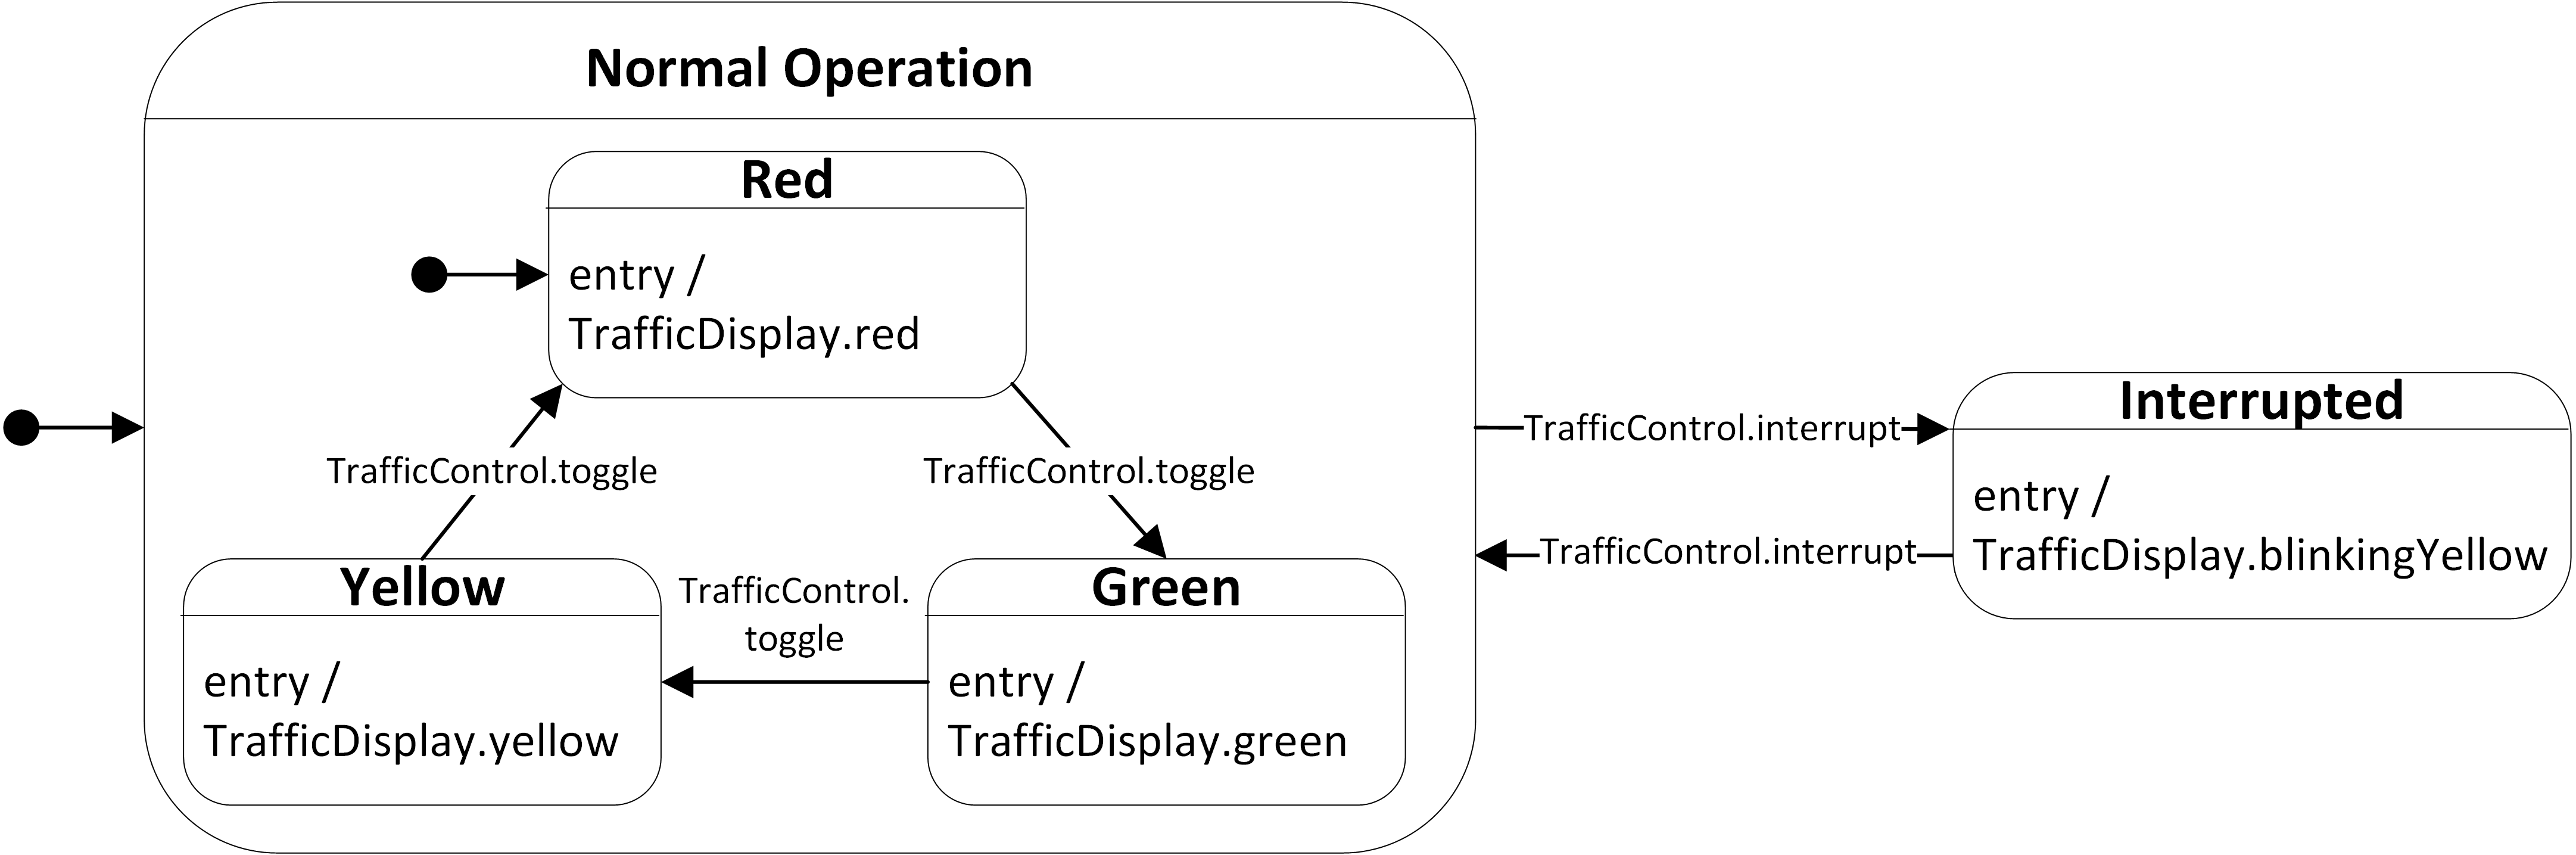
\includegraphics[width=130mm, keepaspectratio]{figures/casestudy_trafficlightexpected.png}
	}
	\fbox{
		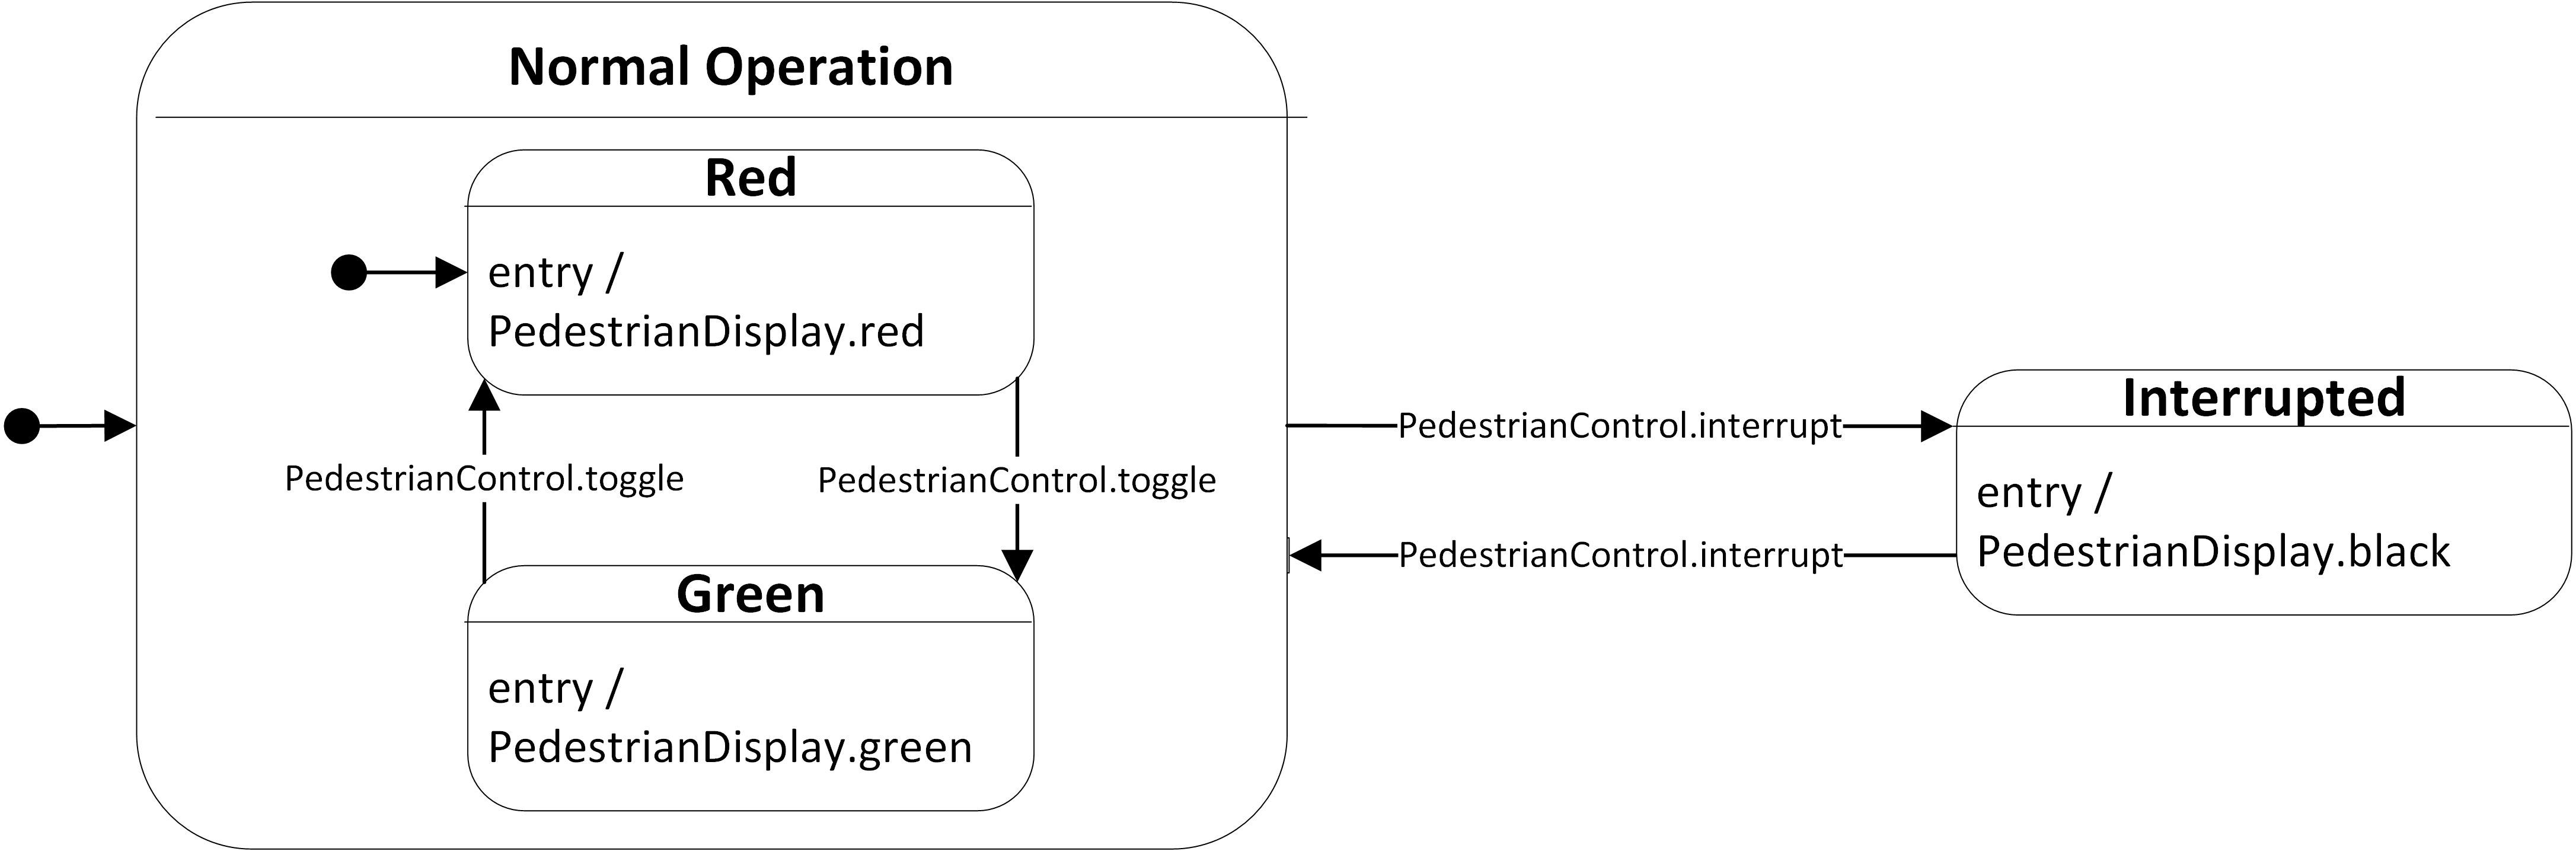
\includegraphics[width=130mm, keepaspectratio]{figures/casestudy_pedestrianlightexpected.png}
	}
	\caption{The expected behavior of the traffic light and the pedestrian light components} 
	\label{fig_casestudy_expecteds}
\end{figure}

\begin{figure}[!ht] 
	\centering
	\fbox{
		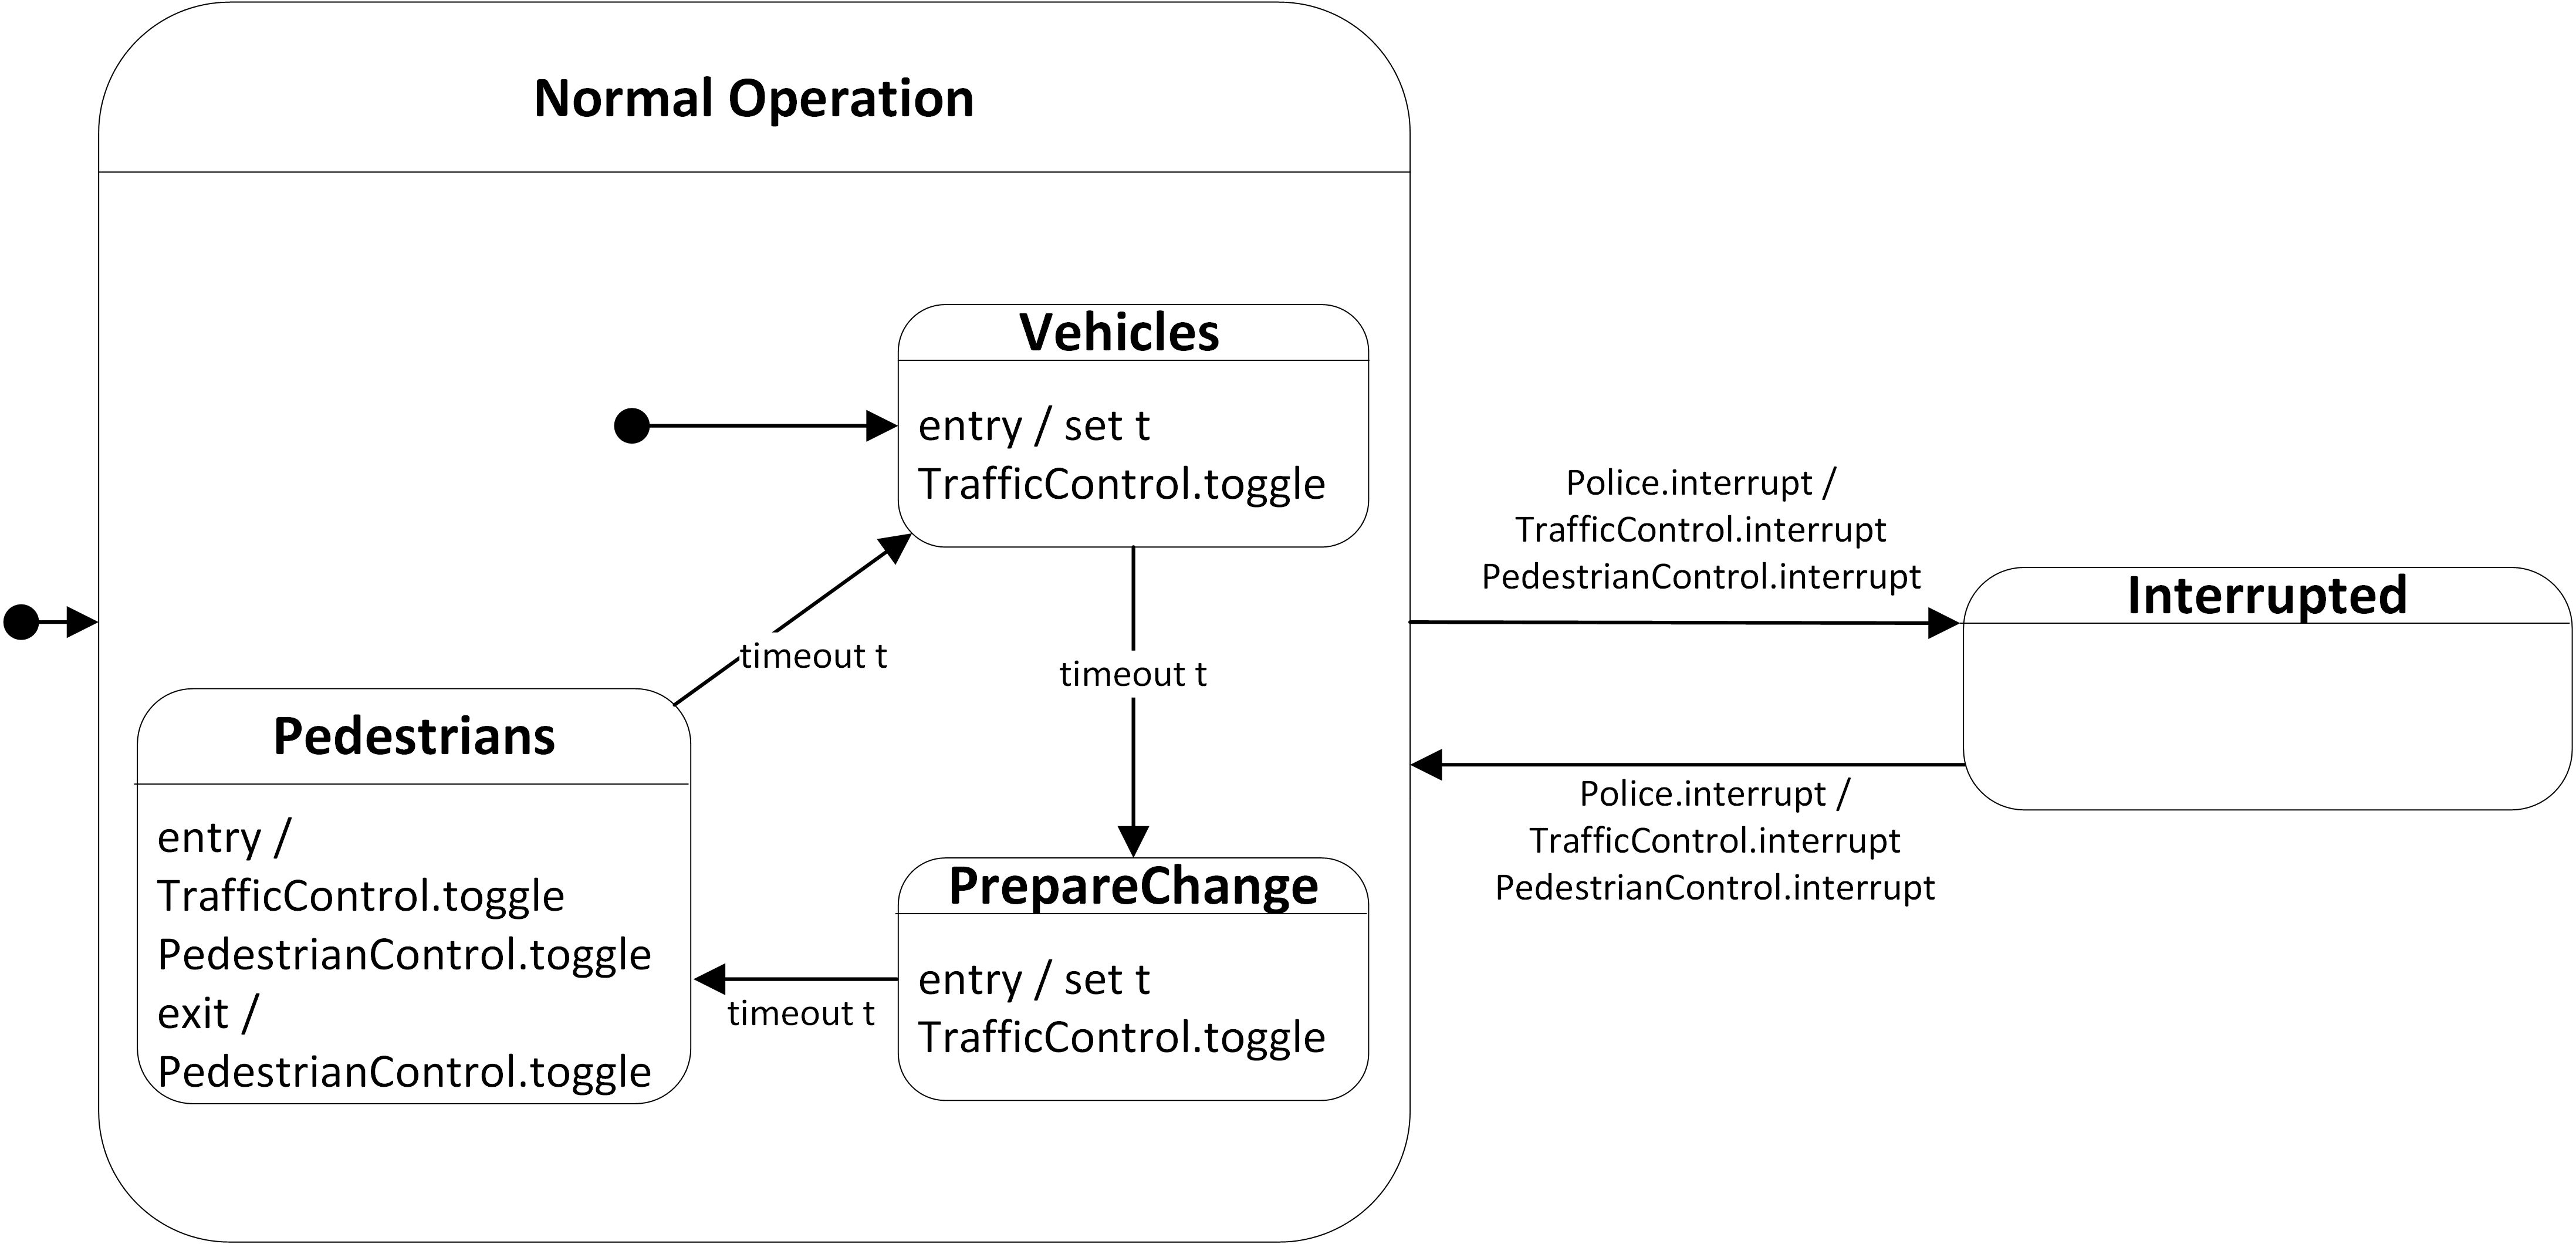
\includegraphics[width=130mm, keepaspectratio]{figures/casestudy_controllerexpected.png}
	}
	\caption{The expected behavior of the traffic light and the pedestrian light components} 
	\label{fig_casestudy_expectedcontroller}
\end{figure}

A képeken az látszik, hogy nem pont ugyanazt kaptuk, de a viselkedés megegyezik, mivel nem tudunk hierarchiát yadda yadda....

A Controller timeoutját a következőképp modelleztük... Időzítést sem tudunk, azonban a usernek lehetősége van kiegészíteni....

Ezek után használhatja a Gamma mindenét a modellekre, etc etc....

[ESETLEG: a teljes rendszert is tanuljuk?]

%----------------------------------------------------------------------------
\section{Future Work} \label{sec_futurework}
%----------------------------------------------------------------------------

